

%\documentclass[11pt, oneside]{article}   	
%\usepackage{geometry}    
%\geometry{letterpaper}                 		
\input preamble.tex
\newcommand{\ig}[2][width=4in]{\includegraphics[#1]{#2}}    		
\usepackage{graphicx}					
\usepackage{amssymb}
\usepackage{pgfplotstable}
\usepackage{float}
\begin{document}

\header {\today}							
\title{Relativistic Electron Momentum}
\author{Ekta Patel \& Brandon Booth-Dunbar}



\section{Abstract}
\begin{em}
%Brandon
\end{em}

\section{Intro}
%Brandon

\section{Theory}

\subsection{Energy}
In Newtonian mechanics, kinetic energy and momentum are given by the following equations of motion:
\begin{equation}KE= \frac{1}{2}mv^2 \end{equation}
\begin{equation} p=mv \end{equation}
\begin {equation}KE=\frac{p^2}{2m} \end{equation}

However, when dealing with particles that are moving at the speed of light, relativistic motion must be considered. When the velocity of a particle,v, approaches the speed of light, c, the equations for energy and momentum become:
\begin{equation} E=\gamma mc^2\end{equation}
\begin{equation} p=\gamma mv\end{equation}
where $\gamma$ is:
\begin{equation} \gamma= \frac{1}{\sqrt{1-(\frac{v}{c})^2}}\end{equation}
Therefore, total relativistic energy of a particle can be written as:
\begin{equation} E=m_0c^2+KE=\gamma mc^2\end{equation}
The first term of Equation 7 represents the rest-mass energy of the particle, which is an electron for the purpose of this lab. Relativistic energy is also commonly expressed in terms of momentum as given by Equation 8:
\begin{equation}E^2=p^2c^2+m^2c^4\end{equation}
\subsection{Momentum and Force}
To measure the momentum of an electron in this experiment, we observe an externally applied magnetic field which can be varied. Recalling the Lorentz force when the velocity vector of a particle is perpendicular to the magnetic field, we have a magnetic force represented as:
\begin{equation} F_{mag}=qvB. \end {equation}
Since we are observing the trajectory of an electron, $q$ can be replaced with the elementary charge, $e$: 
\begin{equation} F_{mag}=evB.\end{equation}
A magnetic force applied perpendicular to the velocity vector of the electron will cause it to be deflected into a circular trajectory from the source, through the slit and into the detector of the apparatus. A relationship between the magnetic field and the momentum of the electron can then be developed by equating the magnetic force of the electron with the centripetal motion of the particle,$F_{mag}=F_c$:
\begin{equation} F_c=\frac{mv^2}{R}\end{equation}
\begin{equation} evB=\frac{mv^2}{R}.\end {equation}
Substituting the Newtonian equation of momentum, $p=mv$, yields:

To make this relation easier to work with, magnetic field is measured in Tesla($1x10^4$ Gauss), radius is measured in meters, and momentum is expressed in units of MeV/c. Substituting the value of an elementary charge and converting to these units transforms Equation 13 to:
\begin{equation} p=300BR\end{equation}
We have derived the expression for momentum is a purely classical way, however, in our experiment, the electrons are moving extremely close to the speed of light so we must validate that this relation for momentum still holds true under relativistic conditions.
\\
\\
The magnetic field hold true under relativistic conditions in this experiment because it is independent of the magnitude of the velocity of the particles. Therefore, the magnetic force is still given by Equation 10. The centripetal force, however, will vary in accordance with the velocity. 
\begin {equation} F_c=\frac{dp}{dt}=\frac{d(\gamma mv)}{dt}=\gamma ma. \end{equation}The acceleration is equal to $v^2/R$, yielding:
\begin{equation}F_c=\frac{\gamma mv^2}{R}.\end{equation} Equation equations 10 and 16 and  recalling the equation for relativistic momentum given by Equation 5:
\begin{equation}p=eBR,\end{equation} which can also be written as \begin{equation} p=300BR.\end{equation} Therefore, we can conclude that the both the classical and relativistic equations of motion result in the same expression for momentum. We can use this result to find the values for a magnetic field that gives the highest count rate to calculate and electron's momentum and energy. 

\subsection{Determining Peak Magnetic Fields}
We use a $^{207}$Bi source, which emits relativistic electrons in the process of changing $^{207}$Bi into an excited state of a $^{207}$Pb nucleus. When $^{207}$Pb decays to a lower energy state, it ejects an electron from the atom. The following figure shows the changes in energy states from the original source of $^{207}$Bi to $^{207}$Pb. \\
\begin{figure}
\begin{center}
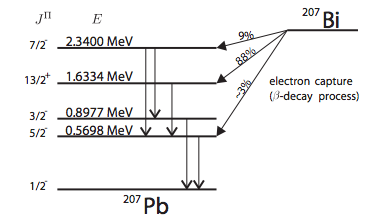
\includegraphics[width=4in]{energylevels.png}
\caption{Transitions of $^{207}$Bi}
\end{center}
\end{figure}
In the first energy conversion, an electron goes from having 1.6334MeV to 0.5698MeV and in the second drop it moves from an energy state with 0.5698MeV to being ejected from the atom where it is no longer bound to an energy state. Thus, $\Delta KE_1=1.064$ MeV and $\Delta KE_2= 0.5698$MeV. \\
\\
Since we know the values for the changes in kinetic energies between energy states, we can solve for relativistic momentum in terms of values that we know:
\begin{equation}KE+mc^2=\sqrt{p^2c^2+m^2c^4}\end{equation}
\begin{equation}(KE+mc^2)^2=p^2c^2+m^2c^4\end{equation}
\begin{equation}(KE+mc^2)^2-m^2c^4=p^2c^2\end{equation}
\begin{equation}\frac{(KE+mc^2)^2-m^2c^4}{c^2}=p^2\end{equation}
\begin{equation}\frac{p=\sqrt{(KE+mc^2)^2-m^2c^4}}{c}\end{equation}
We have proved:
\begin{equation}p=eRB\end{equation}
Where R is the radius of the detector-source apparatus, which we have measured to be .0290m:
\begin{equation}\frac{p=\sqrt{(KE+mc^2)^2-m^2c^4}}{c}=eB(.0290m)\end{equation}
Solving for B, we can estimate our magnetic fields needed to see electron pulses on the oscilloscope for each time an electron is counted:
\begin{equation}B=\frac{\sqrt{(KE+mc^2)^2-m^2c^4}}{ce(.0290m)}\end{equation}
Before solving for B, we must account for the energy lost by each electron due to the k-shell binding energy of Lead, which is $\sim$88keV:
\begin{equation}KE_1=1.064MeV-0.088005MeV=0.975995\end{equation}
Now, we can substitute all of our values into equation 25 to obtain:
\begin{equation} B_1=0.1606T=1.606kG\end{equation}
For the second electron pulse:
\begin{equation}KE_2=0.5689MeV-0.088005MeV=MeV\end{equation}
Once again, using equation 11:
\begin{equation}B_2=0.0979T=0.979kG\end{equation}

It is also important to consider  that the electron loses energy as it travels in the air from the source to the detector. Since we cannot quantify this loss in energy, we must account for it qualitatively while analyzing our  experimental results. With theoretical values for the magnetic fields, we can determine theoretical values for momentum, which we can compare to our results:
\begin{equation}p_1=300RB=300(.0290m)(0.1606T)=1.397 m\cdot T\end{equation}
\begin{equation}p_2=300RB=300(.0290m)(0.0979T)=0.8517 m\cdot T\end{equation}

\section{Experimental Methods}
%Brandon
\subsection{Apparatus}

\subsection{Calibration}
The calibration of the apparatus is the most detail sensitive step in the experiment.  While calibrating the detector system if you set the amplifier too high or the single channel analyzer too low you will get very large background counts from the sensor and will not reliably be able to detect the peaks of electron emission from the Bismuth source.  On the other hand if the discriminator is set too high or the amplifier to low you will not get enough counts to clearly define a peak when you perform your measurements. 
\subsection{Procedure}

\section{Results $\&$ Discussion}

\begin{figure}[H]
\begin{center}
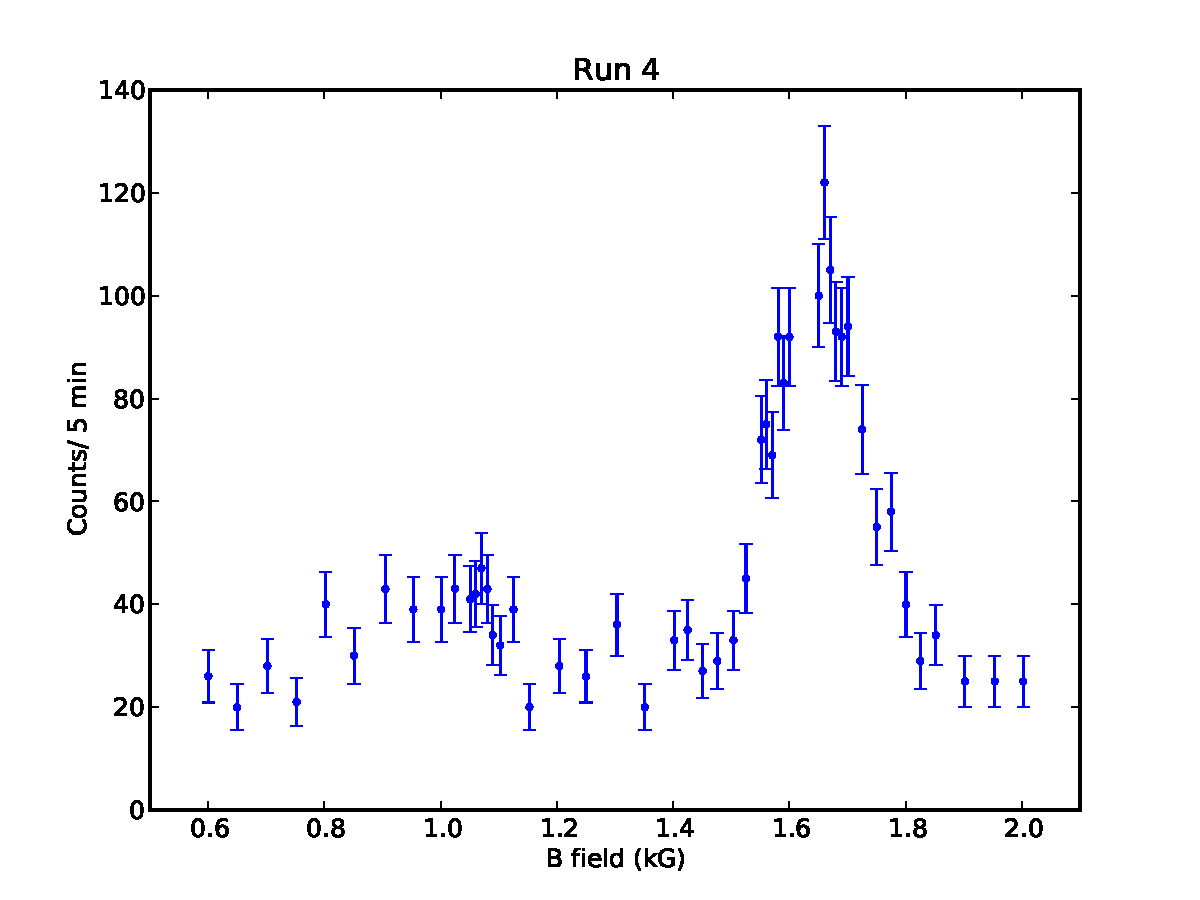
\includegraphics[width=6 in]{figure3.pdf}
\caption{Run 4 of data with extra points taken in smaller magnetic field steps near the theoretical peaks. This data includes the counts from background noise. The error bars in number of counts per 5 minutes are given by $\sqrt{N}$, where N is the number of counts at each value for magnetic field.}
\end{center}
\end{figure}
\begin{figure}[H]
\begin{center}
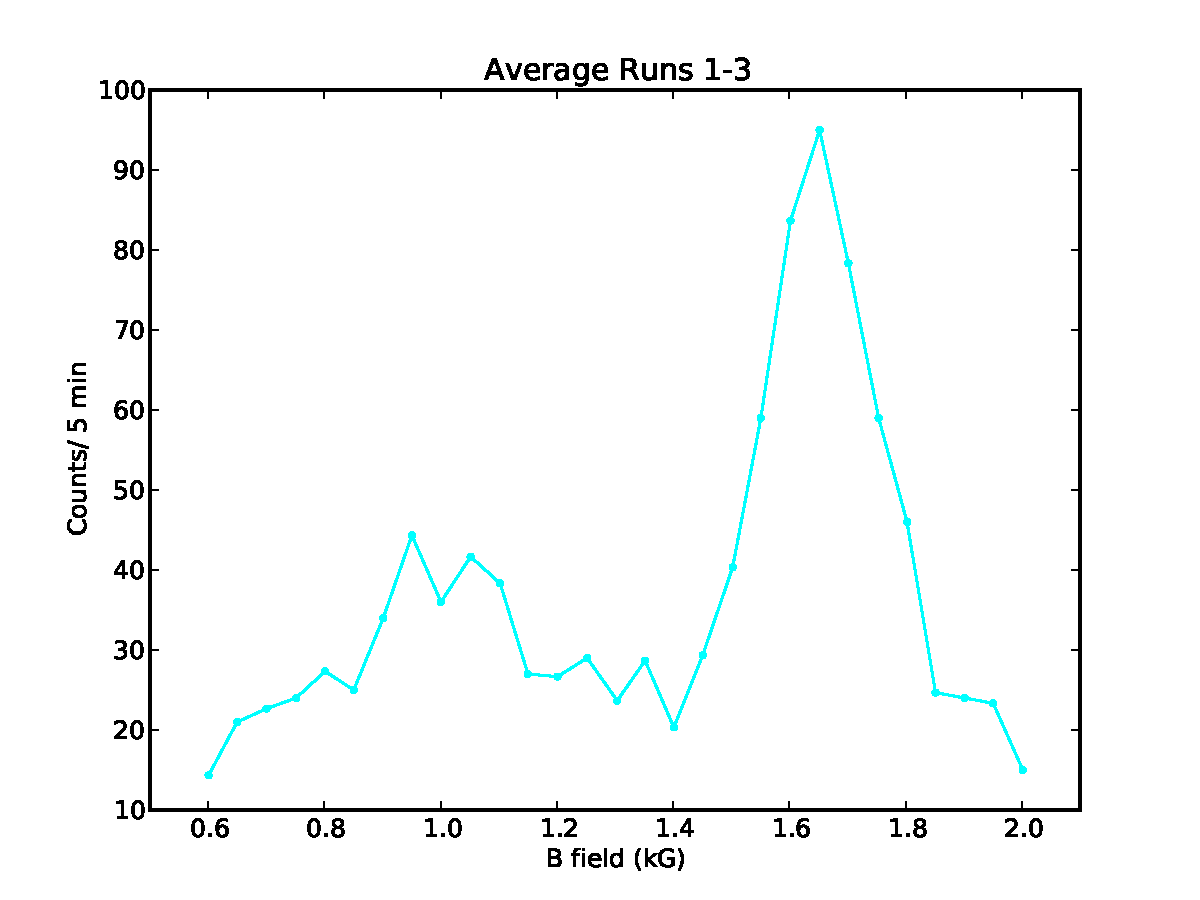
\includegraphics[width=6 in]{figure4.pdf}
\caption{The results of the average  of first three runs of data. Each data set was taken in magnetic field steps of 0.05 kG.This data includes the counts from background noise. The error bars in number of counts per 5 minutes are given by $\sqrt{N}$, where N is the number of counts at each value for magnetic field. }
\end{center}
\end{figure}
\section{Conclusion}
%Ekta & Brandon
%remember to answer all 4 questions here
\section{Appendix}
Data tables and graphs.
\begin{table}[h!]
\caption{Run 1}
\begin{tabular}{|c|c|c|} \hline
Field	(kG)&	Counts	&	Error	\\	\hline
0.6009	&	10	&	3.16	\\	\hline
0.6500	&	26	&	5.10	\\	\hline
0.7009	&	20	&	4.47	\\	\hline
0.7505	&	25	&	5.00	\\	\hline
0.8008	&	32	&	5.66	\\	\hline
0.8507	&	28	&	5.29	\\	\hline
0.9006	&	35	&	5.92	\\	\hline
0.9503	&	44	&	6.63	\\	\hline
1.0002	&	36	&	6.00	\\	\hline
1.0525	&	51	&	7.14	\\	\hline
1.1067	&	40	&	6.32	\\	\hline
1.1498	&	18	&	4.24	\\	\hline
1.2000	&	27	&	5.20	\\	\hline
1.2546	&	31	&	5.57	\\	\hline
1.3061	&	29	&	5.39	\\	\hline
1.3528	&	22	&	4.69	\\	\hline
1.4012	&	20	&	4.47	\\	\hline
1.4503	&	25	&	5.00	\\	\hline
1.5016	&	41	&	6.40	\\	\hline
1.5526	&	50	&	7.07	\\	\hline
1.6018	&	79	&	8.89	\\	\hline
1.6512	&	101	&	10.05	\\	\hline
1.7022	&	74	&	8.60	\\	\hline
1.7554	&	61	&	7.81	\\	\hline
1.8021	&	40	&	6.32	\\	\hline
1.8524	&	24	&	4.90	\\	\hline
1.9022	&	20	&	4.47	\\	\hline
1.9495	&	27	&	5.20	\\	\hline
2.0010	&	15	&	3.87	\\	\hline
\end{tabular}
\end{table}
\begin{table}[h!]
\caption{Run 2}
\begin{tabular}{|c|c|c|} \hline
Field	&	Counts	&	Error	\\ \hline
0.6009	&	14	&	3.74	\\ \hline
0.6500	&	17	&	4.12	\\ \hline
0.7004	&	21	&	4.58	\\ \hline
0.7520	&	21	&	4.58	\\ \hline
0.8014	&	33	&	5.74	\\ \hline
0.8502	&	25	&	5.00	\\ \hline
0.9025	&	37	&	6.08	\\ \hline
0.9505	&	36	&	6.00	\\ \hline
1.0002	&	41	&	6.40	\\ \hline
1.0525	&	38	&	6.16	\\ \hline
1.1004	&	33	&	5.74	\\ \hline
1.1501	&	33	&	5.74	\\ \hline
1.2017	&	29	&	5.39	\\ \hline
1.2506	&	21	&	4.58	\\ \hline
1.3006	&	26	&	5.10	\\ \hline
1.3509	&	35	&	5.92	\\ \hline
1.4012	&	19	&	4.36	\\ \hline
1.4506	&	30	&	5.48	\\ \hline
1.5030	&	39	&	6.24	\\ \hline
1.5497	&	60	&	7.75	\\ \hline
1.6015	&	84	&	9.17	\\ \hline
1.6531	&	92	&	9.59	\\ \hline
1.7008	&	80	&	8.94	\\ \hline
1.7535	&	66	&	8.12	\\ \hline
1.8009	&	58	&	7.62	\\ \hline
1.8501	&	36	&	6.00	\\ \hline
1.9009	&	29	&	5.39	\\ \hline
1.9510	&	22	&	4.69	\\ \hline
2.0019	&	16	&	4.00	\\ \hline
\end{tabular}
\end{table}
\begin{table}[h!]
\caption{Run 3}
\begin{tabular}{|c|c|c|} \hline
Field	&	Counts	&	Error	\\ \hline
0.6006	&	19	&	4.36	\\ \hline
0.6496	&	20	&	4.47	\\ \hline
0.7028	&	27	&	5.20	\\ \hline
0.7513	&	26	&	5.10	\\ \hline
0.8015	&	17	&	4.12	\\ \hline
0.8508	&	22	&	4.69	\\ \hline
0.9008	&	30	&	5.48	\\ \hline
0.9509	&	53	&	7.28	\\ \hline
1.0015	&	31	&	5.57	\\ \hline
1.0498	&	36	&	6.00	\\ \hline
1.1000	&	42	&	6.48	\\ \hline
1.1508	&	30	&	5.48	\\ \hline
1.2014	&	24	&	4.90	\\ \hline
1.2508	&	35	&	5.92	\\ \hline
1.3047	&	16	&	4.00	\\ \hline
1.3518	&	29	&	5.39	\\ \hline
1.4011	&	22	&	4.69	\\ \hline
1.4515	&	33	&	5.74	\\ \hline
1.5027	&	41	&	6.40	\\ \hline
1.5505	&	67	&	8.19	\\ \hline
1.6025	&	88	&	9.38	\\ \hline
1.6518	&	92	&	9.59	\\ \hline
1.7015	&	81	&	9.00	\\ \hline
1.7518	&	50	&	7.07	\\ \hline
1.8043	&	40	&	6.32	\\ \hline
1.8519	&	14	&	3.74	\\ \hline
1.9020	&	23	&	4.80	\\ \hline
1.9514	&	21	&	4.58	\\ \hline
2.0021	&	14	&	3.74	\\ \hline
\end{tabular}
\end{table}
\begin{table}[h!]
\caption{Run 4}
\begin{tabular}{|c|c|c|} \hline
Field (kG)	&	Counts	&	Error	\\ \hline
2.0024	&	25	&	5.00	\\ \hline
1.9532	&	25	&	5.00	\\ \hline
1.9019	&	25	&	5.00	\\ \hline
1.8519	&	34	&	5.83	\\ \hline
1.8253	&	29	&	5.39	\\ \hline
1.8006	&	40	&	6.32	\\ \hline
1.7750	&	58	&	7.62	\\ \hline
1.7503	&	55	&	7.42	\\ \hline
1.7251	&	74	&	8.60	\\ \hline
1.7009	&	94	&	9.70	\\ \hline
1.6902	&	92	&	9.59	\\ \hline
1.6801	&	93	&	9.64	\\ \hline
1.6701	&	105	&	10.25	\\ \hline
1.6603	&	122	&	11.05	\\ \hline
1.6505	&	100	&	10.00	\\ \hline
1.6001	&	92	&	9.59	\\ \hline
1.5903	&	83	&	9.11	\\ \hline
1.5805	&	92	&	9.59	\\ \hline
1.5705	&	69	&	8.31	\\ \hline
1.5602	&	75	&	8.66	\\ \hline
1.5517	&	72	&	8.49	\\ \hline
1.5254	&	45	&	6.71	\\ \hline
1.5038	&	33	&	5.74	\\ \hline
1.4759	&	29	&	5.39	\\ \hline
1.4507	&	27	&	5.20	\\ \hline
1.4249	&	35	&	5.92	\\ \hline
1.4019	&	33	&	5.74	\\ \hline
1.3514	&	20	&	4.47	\\ \hline
1.3035	&	36	&	6.00	\\ \hline
1.2501	&	26	&	5.10	\\ \hline
1.2041	&	28	&	5.29	\\ \hline
1.1528	&	20	&	4.47	\\ \hline
1.1255	&	39	&	6.24	\\ \hline
1.1027	&	32	&	5.66	\\ \hline
1.0896	&	34	&	5.83	\\ \hline
1.0805	&	43	&	6.56	\\ \hline
1.0702	&	47	&	6.86	\\ \hline
1.0606	&	42	&	6.48	\\ \hline
1.0509	&	41	&	6.40	\\ \hline
1.0246	&	43	&	6.56	\\ \hline
1.0011	&	39	&	6.24	\\ \hline
0.9531	&	39	&	6.24	\\ \hline
0.9050	&	43	&	6.56	\\ \hline
0.8511	&	30	&	5.48	\\ \hline
0.8022	&	40	&	6.32	\\ \hline
0.7521	&	21	&	4.58	\\ \hline
0.7020	&	28	&	5.29	\\ \hline
0.6498	&	20	&	4.47	\\ \hline
0.6004	&	26	&	5.10	\\ \hline
\end{tabular}
\end{table}
\begin{figure}[h!]
\begin{center}
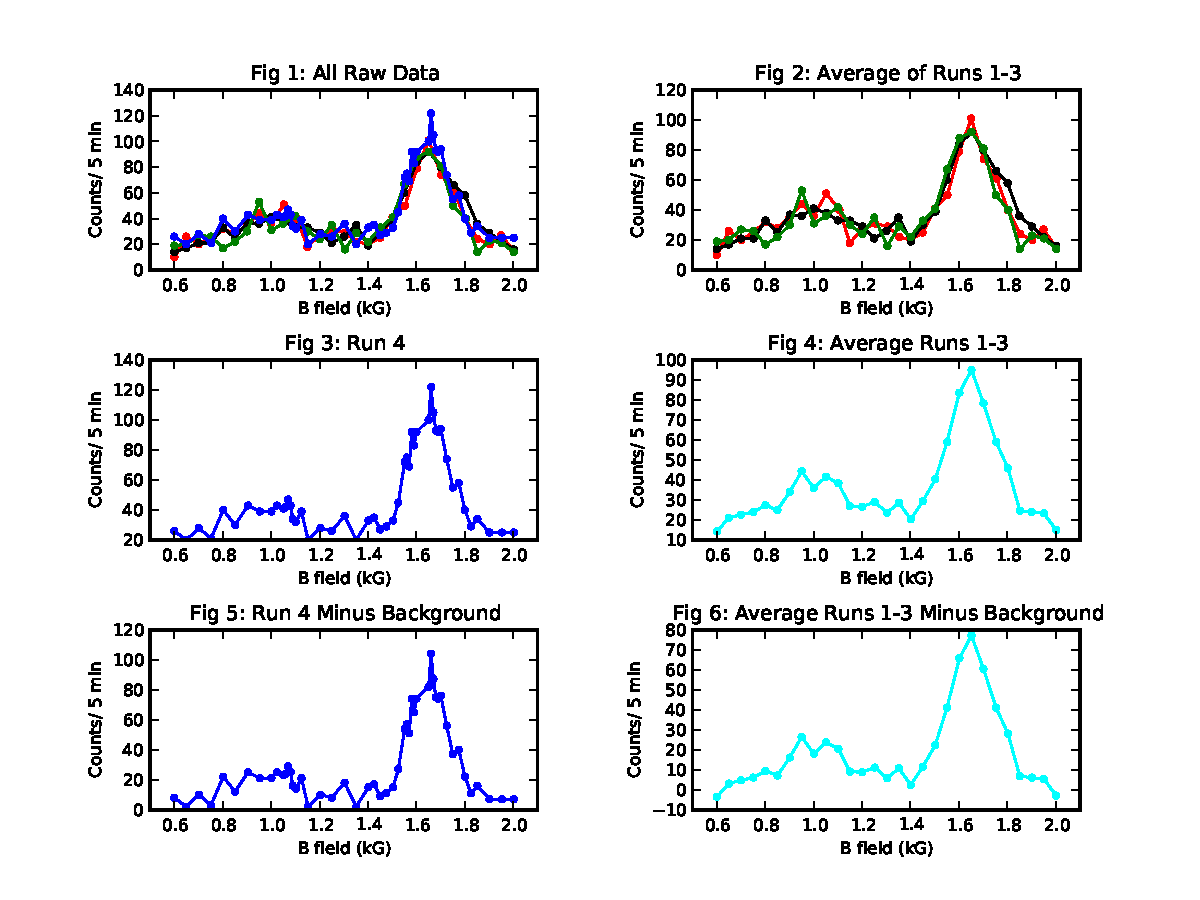
\includegraphics[width=7.5in]{field_counts.pdf}
\end{center}
\end{figure}
%\pgfplotstabletypeset[columns={[index]0,[index]1}, precision=4]{data.txt}
%Referenecs
%Appendix
\end{document}  
